%!TeX program=pdflatex
%!TeX encoding=utf8
%!TeX spellcheck = en_US
%!TeX root = ../../messageVortex.tex
\partepigraph{Limit your inputs to only those that support a certain kind of self-destructive behavior, and you can be cheered with enthusiasm as you drive yourself off a cliff.}{Adam-Troy Castro}
\part{Discussion on Results}
\fxwarning{complete section}

\chapter{Measuring up to the Requirenets\label{sec:reqDiscussion}}
In this section we analyze the level of achievment in respect to the requirements defined in section\ref{sec:requirements}. We will go through each requirement and discuss the level of achievement. In the case of a failure, we highlight the reason for the failure and elaborate on the consequences of the current flaws.

\fxwarning{complete section}


\chapter{Achieved level of anonymity}
\fxwarning{complete section}

\chapter{Weaknesses of the protocol}
\fxwarning{complete section}

\chapter{Further and Missing Research}
\fxwarning{complete section}


In the following chapters, we analyze the protocol thoroughly for fitness of purpose. 

We first apply an analysis of the protocol to identify all pieces of information leaked at all levels.

Then we apply a dynamic attack analysis of the protocol to identify all meta pieces of information leaked during transmission of the protocol such as timing or context between messages. We analyze this by assuming behaving and misbehaving nodes.

We distinguish between passive and active adversaries. Passive adversaries follow the MessageVortex protocol, have unlimited observation capabilities on the network up to layer 4 of the ISO/OSI protocol, and do have unlimited observation capabilities on the transporting layer of MessageVortex. We assume that an observing adversary, as defined in \ref{sec:adversary}, is part of these adversaries. Active adversaries share the capabilities of passive adversaries, but do not follow the MessageVortex protocol. Both adversaries try to obtain valuable information (e.g., message content, metadata such as the communicating peers or message frequencies). 

We then sum up the achieved goals by looking at well-known attacks and analyze the effectiveness of them on the protocol.

At the very end of this chapter, we identify the gaps uncovered by this work.

\chapter{Protocol Analysis}
In this section, we analyze the protocol statically. Looking at a full message, we get the protocol outline, as shown in \eqref{eq:vortexMessage} on page~\pageref{eq:vortexMessage}.

\begin{figure*}[!ht]
	\begin{align}
		VortexMessage                = &\langle \mathbf{MP}^{K^{-1}_{hostN}}, \mathbf{CP}^{K^{-1}_{hostN}}, \mathbf{H}^{K_{senderN}}, E^{K^{-1}_{senderN}}\left(H\left(\mathbf{HEADER}\right)\right)  \nonumber \\
		& \left[\mathbf{R}^{K_{senderN}}\right], \left[\mathbf{PL}\right]*\rangle^{K_{peerN}} \rangle\label{eq:vortexMessage}\\ 
		\mathbf{MP}^{K^{-1}_{hostN}} = &E^{K^{-1}_{hostN}}\left(\mathbf{PREFIX}\langle K_{peerN}\rangle \right)\\ 
		\mathbf{CP}^{K^{-1}_{hostN}} = &E^{K^{-1}_{hostN}}\left(\mathbf{CPREFIX}\langle K_{senderN}\rangle \right)\\ 
		\mathbf{H}^{K_{senderN}}     = &E^{K_{senderN}}\left(\mathbf{HEADER}\right)\\  
		\mathbf{HEADER}              = &\langle K^{1}_{senderN}, serial, maxReplays, validity, [requests, requestRoutingBlock],\nonumber\\ 
		& [puzzleIdentifier, proofOfWork] \rangle \\  
		\mathbf{R}^{K_{senderN}}     = & E^{K_{senderN}}\left(\mathbf{ROUTING}\right)\\ 
		\mathbf{ROUTING}             = & \langle [ \mathbf{ROUTINGCOMBO} ] *, forwardSecret, replyBlock \rangle\\  
		\mathbf{ROUTINGCOMBO}        = & \langle processIntervall, K_{peerN+1}, recipient, \mathbf{nextCP}, \mathbf{nextMP}, \nonumber \\
		& \mathbf{nextHEADER}, \mathbf{nextROUTING}, assemblyInstructions, id \rangle\\
		\mathbf{PL}                  = &\langle \text{payload octets} \rangle *\\ 
	\end{align}
	%\captionsetup{labelformat=empty}
	\caption{Detailed representation of a VortexMessage}
\end{figure*}

\section{Transport and Blending Layer}

\subsection{Analysis of Plain Embedding}
It is undeniable why a file treated with plain embedding is easily identifiable as a broken or tampered file. While the information remains parseable, its content is no longer sensible to a human and thus at least suspect. 

We wanted to know if there is a simple method to detect the modifications of such a file. While most of the analysis method requires the processing of large data sets, we tried to find apparent, non-calculation-intense test methods that were generic. We did not take any content-based characteristics such as ``outline of an image'' or ``resulting spectrum of a sound file'' into account. As our embedding is generic, we searched for a similar detection method.

A property of encrypted ciphertext is the high entropy. We, therefore, used the calculation of the Shannon entropy in bytes as property and tried to show the shift of entropy within the files. This detection method depended very much on the type of file used for embedding. It showed an expected behavior, that file types having in the expected area a similar entropy were not detectable by this method. However, we identified some file types to be unsuitable for plain blending due to their entropy structure.

We analyzed the files by calculating the entropy of blocks 256 bytes with a sliding window over a randomly collected set of images (e.g., the first 100 entries of a file type after searching for ``mouse'', ``cat'', ``camel'', or ``dog''). We did intentionally not filter or eliminate images. Surprisingly, we were able to tell file types apart, were able to identify files with thumbnails or an interlaced structure. We even identified certain specific patterns regarding the producer type of an image (e.g., we could differentiate between pictures scanned or taken by a camera). It was not so much surprising that we were able to identify these features, but the fact that we could see them in entropy data.

\begin{figure*}[ht]
	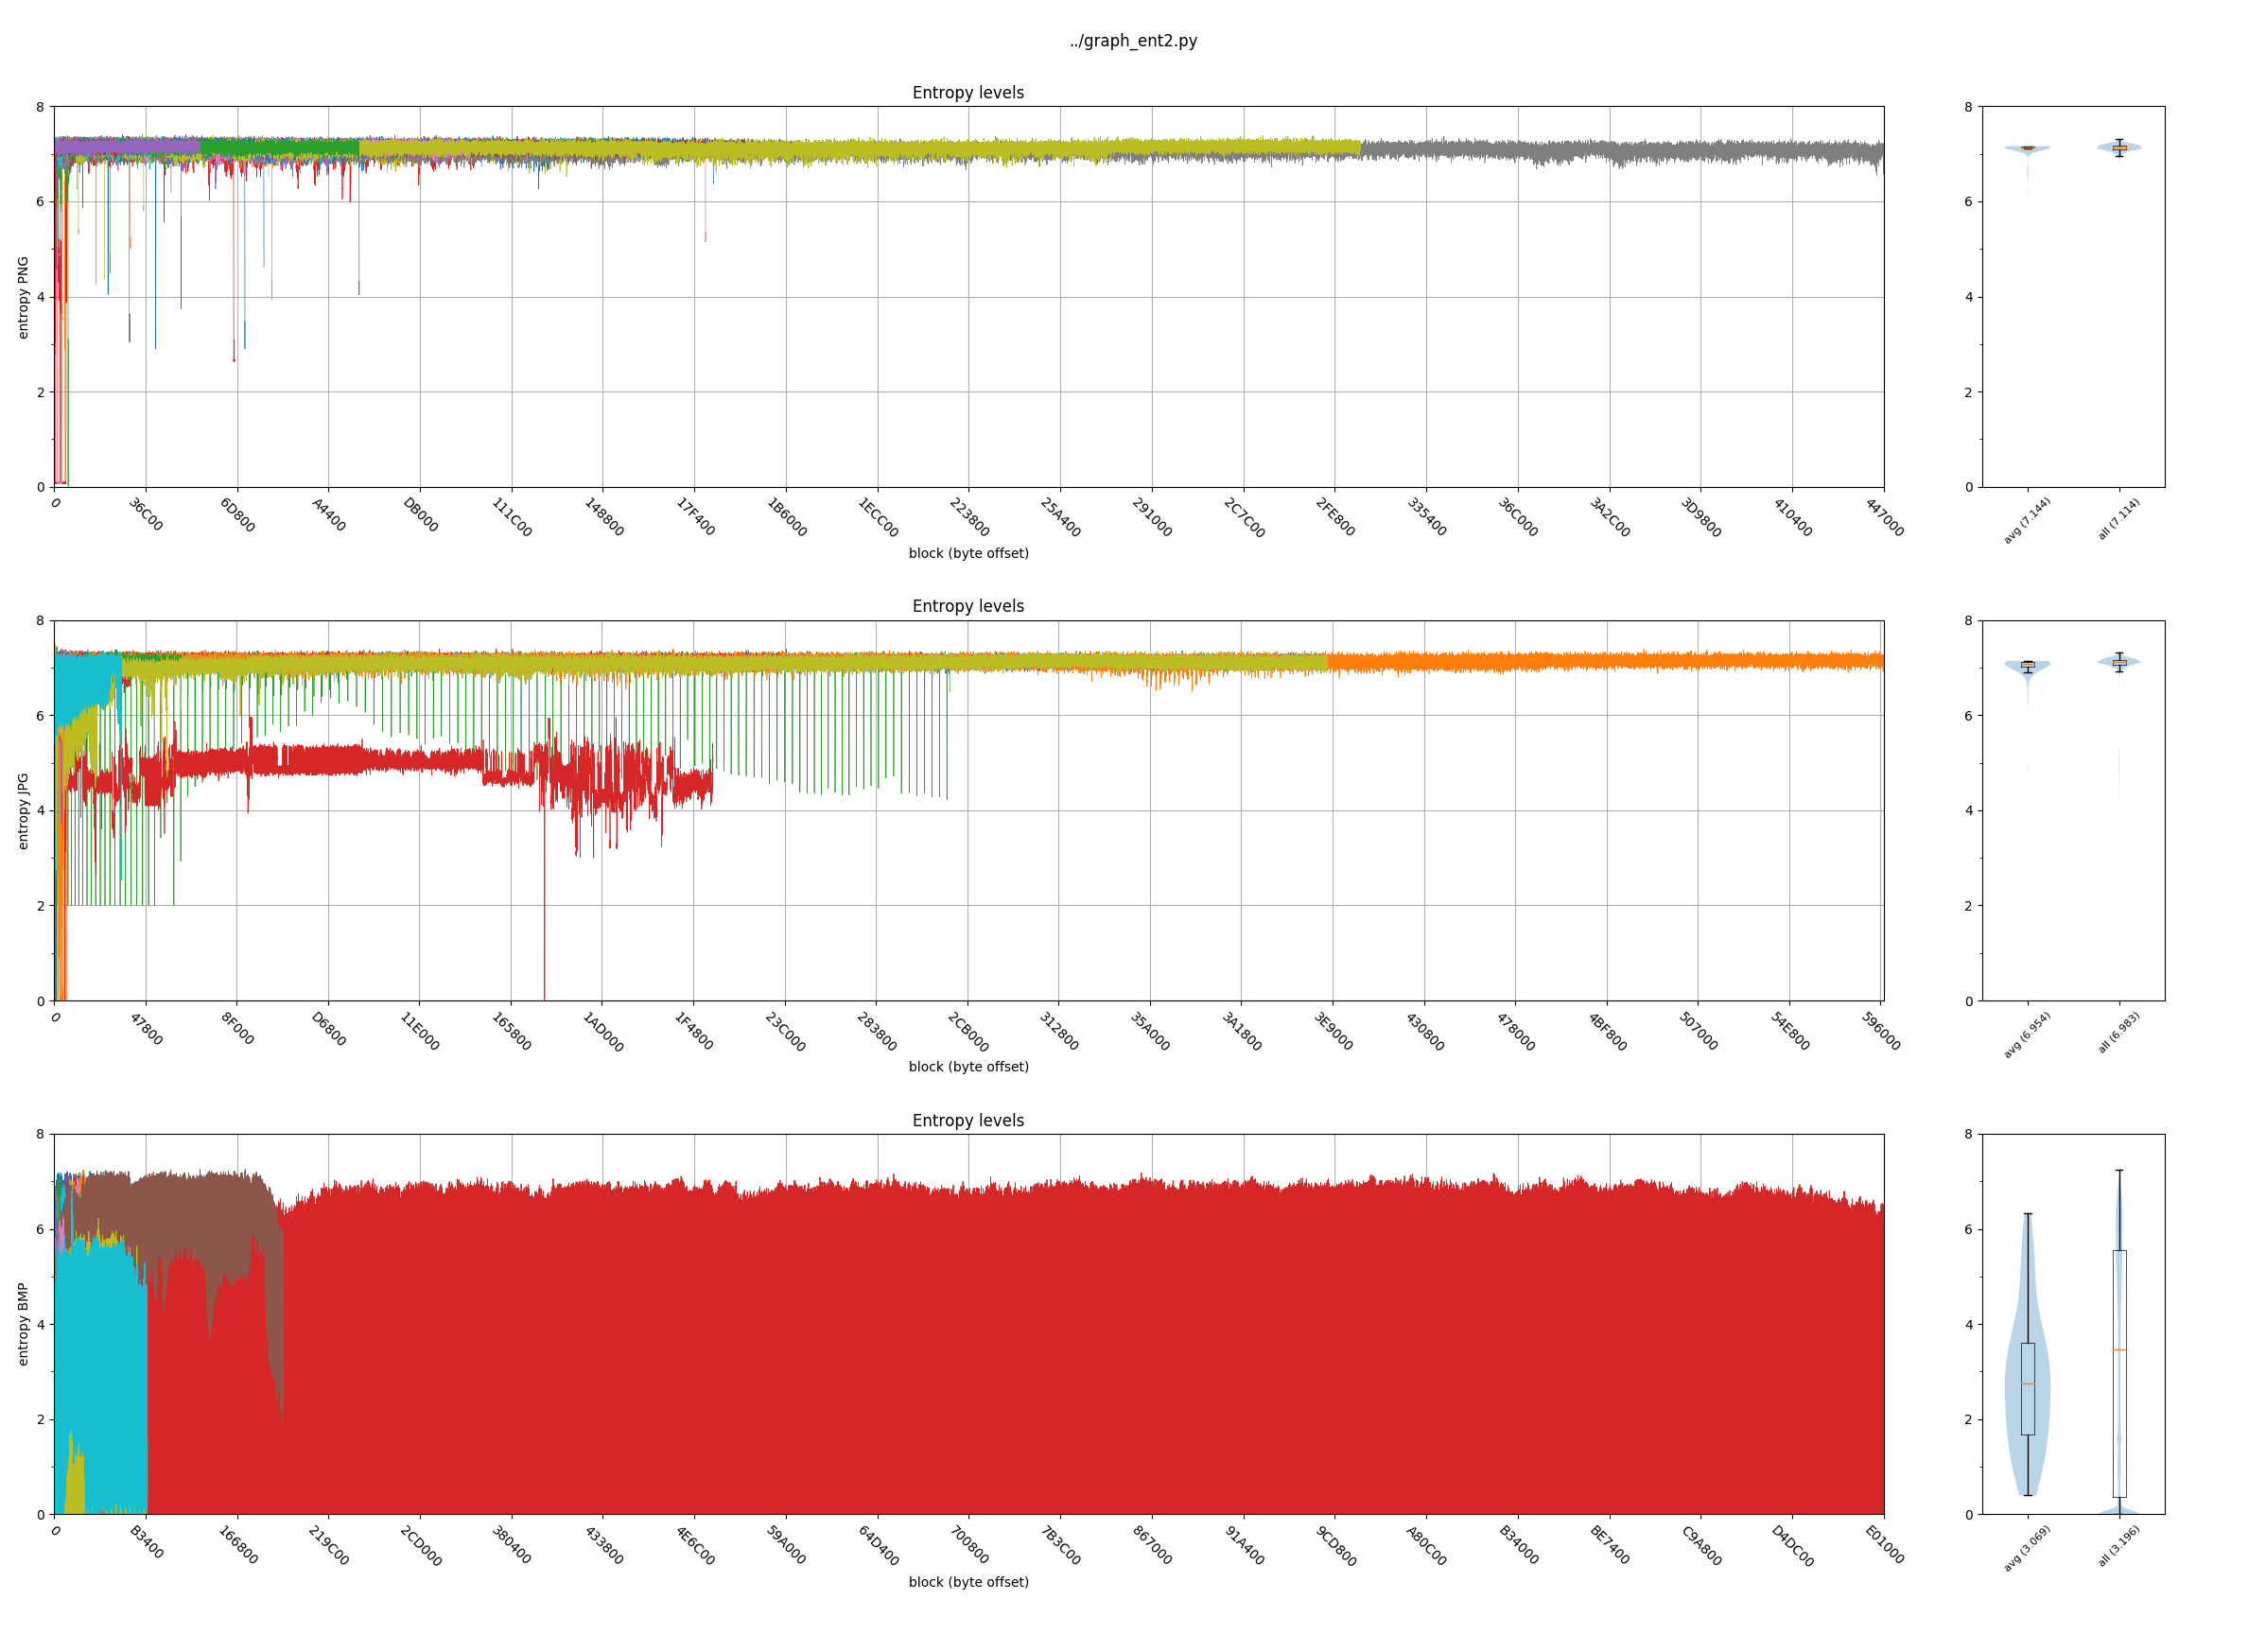
\includegraphics[width=\textwidth]{inc/statanalysis_graph}
	\caption{Distribution Analysis of Different, Common Graphics Formats}
	\label{fig:statGraph}
\end{figure*}

\begin{figure*}[ht]
	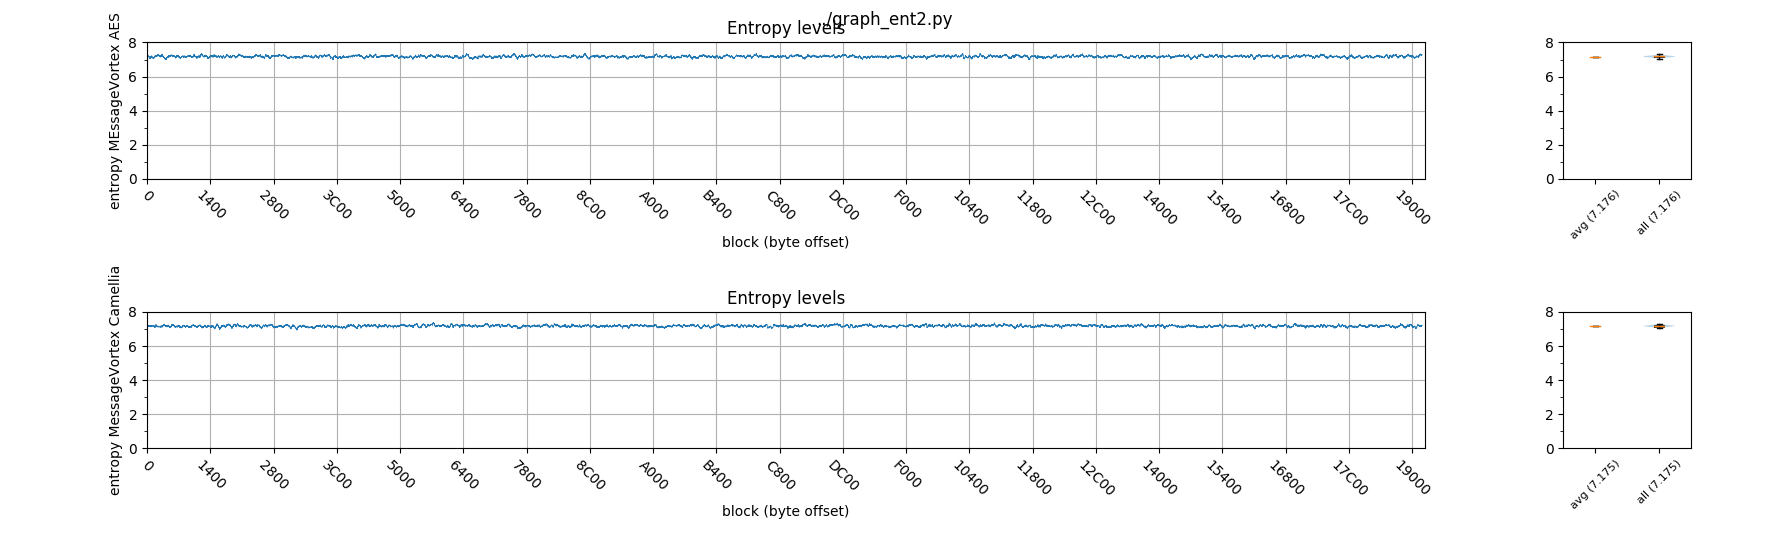
\includegraphics[width=\textwidth]{inc/statanalysis_mv}
	\caption{Distribution Analysis of a MessageVortex Block}
	\label{fig:statMvGraph}
\end{figure*}

We then carried out an analysis identifying the typical entropy and the inner structures. The graphs in \ref{fig:statGraph} show a typical analysis. In that case, we looked at 100 images of each type. We graphed and analyzed their entropy and tested for the suitability of a plain embedding. Table \ref{tab:fileEntropy} lists the average entropy of analyzed file types and makes remarks about the suitability for plain embedding. In practice, we found that most suitable file formats have an entropy of $\approx 7.2$ and an interquartile range (IQR) of 0.15 or less. Furthermore, files should have a big, uniform, the non-structured range containing these characteristics. Such a file has a suitable space for embedding. For reference, Figure \ref{fig:statMvGraph} shows the distribution of typical MessageVortex blocks. We did find that the entropy must be uniformly matched in the case of plain embedding.

\begin{table*}[!ht]
	\centering\tiny
	\begin{tabular}{|l|l|l|l|}\hline
		\diaghead{\theadfont Type Criteria}{Type}{Criteria} & \thead{Avg. Entropy}     & \thead{IQR} & \thead{Remarks}\\\hline
		JPG       & 7.008  & 0.097 & -- \\              
		PNG       & 7.116  & 0.086 & -- \\              
		GIF       & 6.978  & 0.194 & -- \\              
		BMP       & 2.997  & 4.964 & not suitable \\              
		PDF       & 6.660  & 0.282 & Hard to embed due to a very complex inner structure but well suited \\\hline              
		MP3       & 7.076  & 0.091 & -- \\              
		WAV       & 4.777  & 0.927 & -- \\              
		OGG       & 7.104  & 0.093 & relatively easy to embedd. Hard not to break the file structure. \\\hline              
		mpg4      & n/a    & n/a   & good to embedd. Steganography could be applied here easily too. \\\hline              
		zip       & 7.148  & 0.080 & easy to embedd when using ``password protected''  archives \\\hline\hline
		MVaes     & 7.176  & 0.072 & Without length padding as reference encrypted with AES 256 CBC\\
		MVcam     & 7.175  & 0.070 & Without length padding as reference encrypted with Camellia 256 CBC\\\hline
	\end{tabular}    
	\caption{comparison of protocols in terms of the suitability criteria as transport layer}
	\label{tab:fileEntropy}
\end{table*}

When blending into images, BMP showed a strongly varying entropy within a file. A sampling of ten blocks at random position resulted already in detection with a failure rate below 5\%. PNG and JPG files showed to be very robust within the sample. We did not succeed in identifying the MessageVortex blending content based on entropy values. GIF images showed to be unsuitable. Archive formats such as zip files were extremely robust. We were able to embed it into a zip file and marking it (generically) as an encrypted password file. This embedding was genuinely undetectable. However, such embedding may potentially lead to censorship based on blacklisting.

OGG and MP3 are suitable. However, we were able to detect the entropy difference when taking extreme dense samples. These formats may, however, be suitable for not yet standardized forms of steganography. While PDF has low entropy and a high IQR typically, some parts of the files are very well suited for embedding. Plain embedding with knowledge of the format was even possible without affecting the visual result of the file.

We could show that with an approach based on Shannon entropy, we may identify plain embedded MessageVortex blocks in BMP and WAV files. Most of the file formats analyzed were performing well. They required a multitude of samples to detect the presence based on the entropy property.

All movie formats were performing similarly to jpg and PNG. However, due to the very complex structure with scattered blocks, they seem to be unsuitable for plain embedding. They are, however, strong candidates for steganography.

\subsection{Identifying a Vortex Message Endpoint}
Depending on the blending method, a single, identifiable message is sufficient to identify a VortexNode. Detectability depends on various factors, such as:

\begin{itemize}
	\item Broken internal file structure (due to plain blending)
	\item Uncommon high entropy in a structureless file
	\item Unrelated message flow (see \cite{oakland2013-parrot})
	\item Non-human behaviour on the transport layer (e.g., message traffic 24x7)
\end{itemize}

If an endpoint is successfully identified, then all peering endpoints of the same protocol may be identified as well by following the message flow. This does, however, not enable an adversary to inject messages as the host key is not leaked. 

Assuming a global observer as an adversary and unencrypted traffic, he might discover the originating routing layer and thus identify it as Vortex node by following traces of the transport layer. In most protocols, however, this address is spoofable and not a reliable source for the originating account.

\section{Senders routing layer}
A sender may have some knowledge about the Routing block size and may, therefore, guess the complexity of the routing path. He is, however, unable to gain any additional information such as time of travel or number of hops until the target.

\section{Intermediate node routing layer}
An intermediate node does know all the operations applied and the immediate next hop. It does learn the routing addresses of the immediately following endpoints but is unable to use these endpoints. This is because he has no means to get the host key required to communicate.

If a routing block is repeated, a router may identify the routing block as repetition. Identifying the repetition of a block can be done by looking at the serial number of replay protection. We then may give a rough estimate of the message size by comparing the payload chunks. This estimate is, however, very rough as it is bounded by the block size of the symmetrically applied encryption.

\section{Security of Protocol Blocks}
To analyze the security of the protocol, we first go through all protocol blocks. After that, we will look at the possibilities of block recombinations and how to gain data or services based on such behavior. 

Assuming plain embedding, the presence of a chain of blocks may leak an existing VortexMessage. At the moment, the protocol expects at the offset and the size of the bytes to be skipped to the next block. The encoding does not assume an end of the chain marker as such a marker would make the design identifiable. As an encoding scheme, a variable byte length has been chosen. This guarantees that any file will always result in a valid chain of blocks and thus not leak such a presence.

The entropy of the only two blocks in this stream (MPREFIX and InnerMessageBlock) is comparable as both blocks are encrypted. Both blocks are encrypted and feature a similar entropy. The blocks follow each other without any delimiter. This results in a continuous stream of data with constant properties. 

To avoid repeating patters at the beginning of streams due to reused identity blocks, a MURB must provide sufficient peer keys and prefix blocks. A VortexNode may, however, refuse to process MURBS (only accept maxReplays equal to 0).

All blocks of InnerMessageBlock are protected by the peer key $E^{K_{peer}}$. The forward secrets in all blocks except the payload blocks make sure that the recombination of blocks does not work for an adversary. To be successful, an adversary requires to know the forward secret of the next hop.

To keep the secrets of the next hop, hidden from the host assembling the message, the subsequent header and the routing block are protected by the sender key $E^{K_{sender}}$. A message assembling node is, therefore, not even capable of creating its own messages to an unknown node as the hosts' public key $E^{K^{1}_{host}}$ is not derivable from a message.

Therefore, a routing node is not able to assemble messages for a specific host on the base of a routed message only. A routing node does not gain any additional knowledge except for the locally executed operations, the number of messages of the ephemeral identity, the size of messages of any ephemeral identity, the sending IP of a received VortexMessage and the transport endpoint address of any receiving endpoint. The most critical information is endpoint data, as all other data is unrelated to the original message (sender recipient and size). This information becomes absolutely crucial if assuming a censoring adversary. Therefore, a sender in a jurisdiction where the use of MessageVortex is deemed illegal must use only trusted nodes within the jurisdiction and at least for the first hop outside the jurisdictional reach of an adversary.

\chapter{Dynamic Attack Analysis}
In the dynamic analysis, we reach out to an active adversary. An active adversary modifies traffic in a non-protocol conformant way, or misuses available or obtained information to disrupt messages, nodes, or the system as a whole.

\section{Attacks against the vortex system itself}
An active adversary may attack the transport layer. Most of the transport layers are not able to react upon message flooding. Therefore, it is easy to attack a transport layer with a flooding attack, such as a distributed denial of service (DDoS) attack. Due to the nature of the protocol, we are unable to create additional protection on the transport layer as such modification would require a modification of the transport layer. The Vortex Message format itself is, however, crafted in such a way that only minimal effort is sufficient to get the involved parties of a transmission. The Operations $ K_{msgN}=D^{K^{1}_{host}}\left(P\right)$ and $HEADER=D^{K_{msgN}}\left(H\right)$ are sufficient to identify message senders. Unknown Senders may be discarded without further processing. Known senders may be identified as legitimate and processed further. Known misbehaving identities and message duplicates may be discarded. 

\subsection{DoS Attacks against the System}
An active adversary may not follow the protocol and modify any parts of the message. The following paragraphs reflect different kinds of behavior and how they affect the messages and the system as a whole.

An adversary may not follow the blending specification. If he uses a less secure specification, an independent third party observer may follow traffic. This is not sensible as such a node may send all the knowledge to such a collaborating node directly. In the case of a  target node not supporting the chosen blending method, the partial message path becomes interrupted. A possible redundancy in the path may recover the message from such a case.

\subsubsection{DoS by Traffic Replay}
Traffic replay is a common way to highlight traffic in many systems by replaying the same traffic and increase the signal to noise ratio of a system. In our case, we can use the replay of a VortexMessage block to increase the traffic to a node. After decoding the header, a MessageVortex node identifies the block as a repeated block and rejects further processing. 

An adversary may replay blocks with varying content. This will not result in a DoS attack as the quota is not decreased on replayed messages (see Figure~\ref{fig:msgRecvProcessing}).

\subsubsection{DoS by Traffic generation}
An adversary may first collect identities and quotas and use them later in a coordinated attack to force the node processing. The adversary may increase the impact by using large payloads and processing them in a costly manner. A possibility is to make extensive use of $addRedundancy$ or encryption operations. Furthermore, an attacker may attack the memory by distributing the message throughout the workspace to exhaust the routers' runtime memory.

As a router is free to process the operations of identity, he may discard an ephemeral identity and all associated resources at any time. Misbehaving or suspected misbehaving nodes may, therefore, be stopped. On the other hand, we are unable to prevent an adversary from allocating new identities. We may, however, work with multiple local host keys and distribute them according to the trust. A known party or someone trusted by them might receive a key different from a publicly advertised key. This identity key may be dropped at any time and distributed to further parties again with an identity update. We may even subdivide trusted parties into several groups by updating them with different new host keys to identify misbehaving routers without knowing them. 

\subsection{Attacking a single ephemeral Identity of a MessageVortex Node}

\subsubsection{Denial of Service by Exhausting Quotas or Limits}
A malicious node may try to exhaust quotas or limits. As we do trust in the sender and recipient, all other nodes do not know the forward secrets used in the message. The options for an adversary are then as follows:

\begin{itemize}
	\item Resend a MURB (with different content) as often as possible to exhaust message and transfer quota. 
	\item Create intentionally huge, incorrect message content to exhaust transfer quota.
\end{itemize}

\subsection{Attacking Sending and Receiving Identities of the MessageVortex System}
The most valuable goal of an adversary is breaking an entity's anonymity or monitor their traffic by the content or the metadata. In the following sections, we analyze the possibility of 


\subsubsection{Traffic Highlighting}
Traffic caused by a routing block may be observed to a certain extent on a statistical base. A node may generate bad message content of exceptionally large or small nature. This might potentially highlight messages involved in message routing using no split or relative split operations as well as addRedundancy operations.

\subsection{Recovery of Previously Carried Out Operations}
It is crucial that an adversary is unable to recover parameters of a previously carried out operation. We analyzed though the protocol operations carefully to be sure not to leak any of the parameters. Some operations leak apparent data such as an encryption operation with a block cipher does typically leaks its block size. This has, however, been classified as invaluable data as the block size does not result in any information gain usable for attacking the system or narrowing down efforts. In figure \ref{fig:randomBlockAnalysis}, we can show that the parameters are visible. We took the same 10kb block and treated it with all possible combinations of operation parameters. The image shows that there is a possibility of guessing the parameter with a high probability. For guessing the average Monte Carlo Pi and the average Shanon entropy in bits per byte were already sufficient. The results got a bit less clear when applying the same operation to random blocks while doing the analysis. 

We have, however, found a flaw in the$addRedundancy$ operation. When applying this operation to an encrypted block, the entropy of the resulting block leaks some of the parameters of the operation. As a result of this finding, we added a custom padding and an additional encryption step. The repeated analysis showed that the operation does no longer leak these parameters through this channel.


\section{Achieved Anonymity and Flaws}
\subsection{Measuring Anonymity}
It is tough to measure anonymity, as it involves many uncontrollable factors. We may, however, control the degree of anonymity according to the number of involved parties. Assuming a sender knows the complete message path, including all operations carried out on any untrusted node a message travels through, the anonymity is maxed to the number of involved nodes $n$, excluding the sender nodes. This degree of $n-1$ may be further reduced if all well-known ``routing only'' or at least ``routing mostly'' nodes are reduced. Under these harsh assumptions, the set may be reduced to the potential set of ``well known'' recipients of a message.

We have to differentiate between several problems. An adversary has to identify the participants of an anonymity system. Then he has to identify members of a message or a communication anonymity set. Starting from there, he has to identify message flows and detect senders and receivers of messages within an anonymity set (which is not doable in all cases). If any adversary achieves this, we have to consider the anonymity to be broken. Depending on the degree of anonymity required, which is influenced by external factors, the participation in any or a small enough set may be sufficient to suffer consequences.

\subsection{Attacking Routing Participants}
While very hard in our case as we do not have ``dedicated'' anonymization infrastructure, It might be possible to identify members of the routing network. This due to flaws in the blending layer. While it is possible to scare off or block members of a routing network. It is far harder in a network where the members are mobile. Any user may change at any time the identity, including the endpoint, without losing its known peers. This unique property makes the participating entities very mobile and allows them to switch servers at any time without losing contact with peers for subsequent communication.

Routing participants may be identified either by publicly available information (e.g., published routing address) or by identifying unique properties of the protocol. Transport layer provider may then be forced to deanonymize the customer related to the account (if possible), or the relating account on the transport layer may be blocked. 

To counter a possible threatening deanonymization, a MessageVortex node owner must maintain anonymity towards the transport layer provider. Nowadays, this is easily done in the XMPP protocol. The account is typically not linked to any subsequent user information, such as telephone or email. Email accounts are more restrictively regulated. Providers providing accounts without registration of phone numbers or subsequent email addresses do exist (e.g., Yandex) but are rare. In both cases, a user might be identified by its IP address. This is why concealing its IP address while connecting to the transport layer is an advisable practice. Using Tor when accessing the transport layer may suffice to do so. The anonymizing service has to be strong enough to conceal the IP. The protection of the traffic itself is not required as it is already protected.

\subsection{Attacking Anonymity through Traffic Analysis}
As traffic and decoy traffic and decoy traffic are chosen by the creator of the routing block, frequency patterns cannot be detected, unlike the router did create them. The same applies to message sizes and traffic hotspots. When reusing the same routing block, eventually message sizes or general estimates such as ``bigger'' or ``smaller size'' can be made.

For an evil routing node, even paired with a global observer, it is hard to extract any useful information. An adversary might identify all messages following through it as messages of the same true identity. As ephemeral identities are short term identities, this is of limited values. By monitoring the endpoints used by an ephemeral identity, we might calculate a ``likelihood of matching'' for two ephemeral identities. Luckily this is not doable without allowing a high factor of uncertainty. This matching does not improve when combining multiple ephemeral identities over time. The matching might slightly improve when trying to match ephemeral identities on different routing nodes. Making strong statements about those likelihoods is not possible as we did intentionally not define a specific behavior. We may safely say that the possibility of deanonymization is degrading if using short-lived ephemeral identities.

The knowledge a node may gain from ephemeral identities is minimal. The ephemeral identity is created by a node unknown to the receiver of the request. The only thing we know is what node was adjacent when creating the ephemeral identity. As the creation of an ephemeral identity is not linked to any other identity or ephemeral identity relationship between ephemeral identities on two nodes cannot be established. If two adjacent nodes cooperate when processing two linked ephemeral identities, no additional knowledge may be won. If two collaborating nodes have one or more non-collaborating nodes between them, they lose all linking knowledge due to the non-collaborating nodes. 

Operations have been carefully crafted to leak as little information as possible. Being able to encrypt or decrypt a payload block does not leak any information. The data processed may be true message traffic or decoy as we do not know what the nature of the received message was. If an RBB avoids repeating patterns of blocks on nodes, it is not possible to link ephemeral identities of two non-adjacent nodes. Repeating patterns may arise, for example, if a block $pb_1$ is decrypted and re-encrypted on two nodes. In this case, both nodes may match the message as it contains the same content between the operations.

\begin{eqnarray*}
	\text{node f:}\\
	& pb_2 & = D(pb_1\\
	& pb_3 & = E^{K_t}(pb_2)\\
	\text{node f+1:}\\
	&.\\
	&.\\    
	\text{node f+x:}\\
	& pb_4 & = D^{K_t}(pb_3)\\
\end{eqnarray*}

In this example the patterns of $pb3$ and $pb_4=pb_2$ are two patterns repeating on non-adjacent nodes. The same conclusions are even more valid for splitting operations. These two operations should be regarded as helpers for the $addRedundancy$ and $removeRedundancy$ operations. These operations may be used to generate decoy traffic or to destroy data without knowledge of doing so of the processing node. If we process a function $addRedundancy_{2 of 3}$, any of the output blocks contains the input payload, and any two of them may be used to recover the data. At the same time, an operation $removeRedundancy_{2 of 3}$ may be successful or not. The node is unable to differentiate between the two states. The padding applied and the unpadded encryption makes it impossible to judge upon success or fail of an operation.

As the communication pattern is defined by the RBB and not always the same, it is hard to judge on the security. We may, however, look at some generic examples and show that we can achieve the goals byzantine fault tolerance, privacy and unlinkability, and anonymity. Figure~\ref{fig:messagePaths} shows a sending node $s$, a series of routing nodes $n_i,j$ assembled to routing chains. Furthermore, we have a $r$ for which the message is destined and a set of nodes $a_k$ building the anonymity set. Neither the number of chains $j$ nor the length of the chains $i$ is relevant. A node or a sequence of nodes may be part of multiple chains. By normalizing a path into such a form, we may at least analyze some properties of the protocol. We furthermore have to keep in mind that we trust sender $s$ and receiver $r$. Any possible routing block may be reduced to this scheme if knowing the exact building instructions applied by the RBB.

%%%%%%%%%%%%%%%%%%%%%%%%%%%%%%%%%%%%%%%%%%%%%%%%%%%%%%%%%%%%%%%%%%%%%%%%%%%%%%%%%%%%
%%% Manual float placement
%%%%%%%%%%%%%%%%%%%%%%%%%%%%%%%%%%%%%%%%%%%%%%%%%%%%%%%%%%%%%%%%%%%%%%%%%%%%%%%%%%%%
\begin{figure}[ht]
	\centering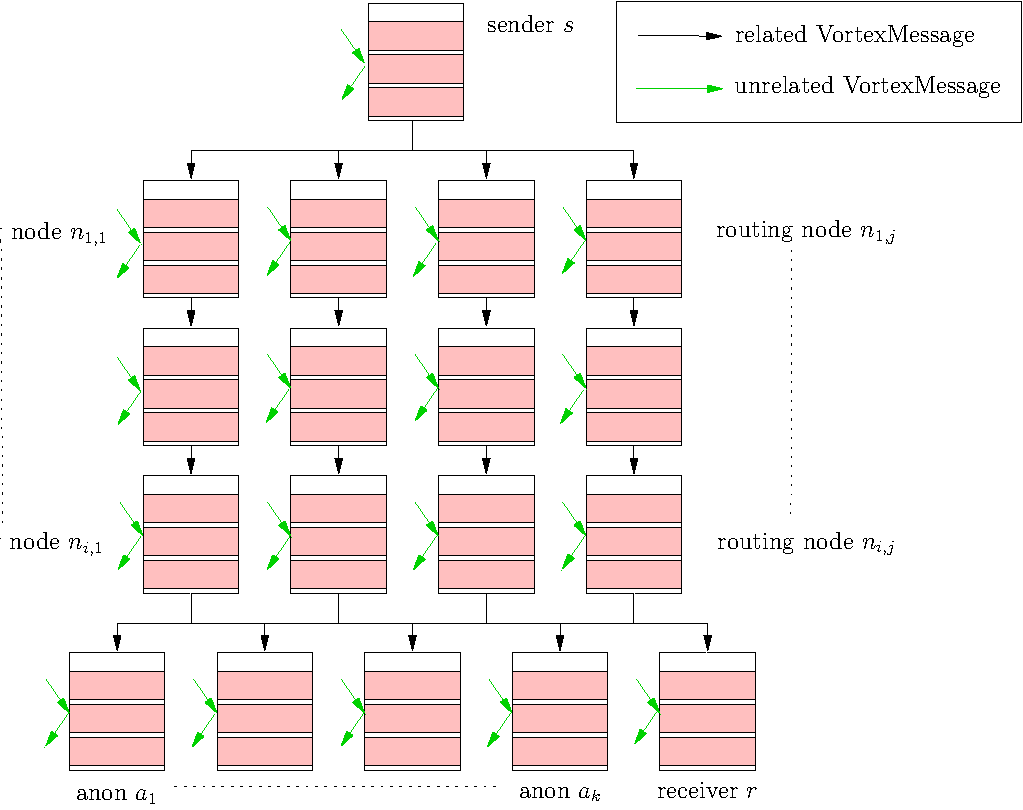
\includegraphics[width=0.7\columnwidth]{inc/messagePaths}
	\caption{A possible path of a VortexMessage}
	\label{fig:messagePaths}
\end{figure}

We have to consider the fact that two adjacent nodes collaborating may build one combined workspace executing all operations. They are, therefore, able to link all operations of these two adjacent nodes and follow all incoming and outgoing paths. We, therefore, may assume that two adjacent nodes or an uninterrupted series of collaborating nodes may be substituted by one node.

So a routing node $n_{1,}$ may not know if a \emph{VortexMessage} received from $s$ is the result of processing another message or the message has been injected on node $s$. Furthermore, if $s$ was acting as a routing node, it successfully unlinked the message from any previous node. The sending node $s$ may send a message by first employing an $addRedundancy$ operation or splitting and encrypting the message. Each path through the streams has then not enough information to rebuild the combined message. If employing an $addRedundancy$ operation, a receiver $r$ may recover a message, if sufficient paths through the routing nodes were acting according to the protocol. Paths with misbehaving nodes may eventually be identified depending on the number of redundancy operations. Assuming that the RBB included proper padding Information for the receiver $r$, the receiver may identify what set of \emph{VortexMessages} leads to the original message due to the padding applied before the $RS$ function. So if sufficient paths, depending on the chosen operations at $r$, provide correct data, we may recover nodes misbehaving in our paths. If one node in a path is not collaborating with adjacent nodes in the path, the path of the \emph{VortexMessage} becomes unlinked as previously shown with sender $s$. If multiple paths are used, all paths must have at least one honest node to unlink the message. 

If all nodes in the anonymization set $a_1$\ldots$a_k$ are honest, any preceding node may not know whether the message ends at that node or the message is just routed through an honest node. Even if some of the anonymization nodes are not honest or collaborating with an adversary, the anonymity set may be reduced in size, but the receiver is still part of the anonymity set spanning the honest anonymization nodes. So, we have shown that depending on the chosen routing block, anonymity, unlinkability, and fault tolerance against a misbehaving node may be achieved. AN RBB may furthermore send additional \emph{VortexMessages} to suspected misbehaving nodes. If misbehavior is reproducible within an ephemeral identity, the RBB may identify it by picking up parts of the previously sent message and comparing them to an expected state. An RBB may even introduce message paths leading back to the RBB itself. Such a message path may allow observation of the progress and success of the message delivery.

\subsection{Attacking Anonymity through Timing Analysis}
Timing is under full control of the routing block builder. No information can be derived from the timing. This is even the case if a routing block is reused. The precise timing on the network depends additionally on other factors, such as delaying through anti-UBE or anti-malware measures or delays through local delivery between multiple nodes.

\subsection{Attacking Anonymity through Throughput Analysis}
Increasing the throughput to highlight a message channel is not possible since the replay protection will block such requests. It may be possible for a limited number of times by replaying a MURB. This is one of the reasons why the usage of MURBs is discouraged unless necessary.

\subsection{Attacking Anonymity through Routing Block Analysis}
The routing block is cryptographically secure. The size of the routing block may leak an estimate about its inner complexity. It does not reveal any critical pieces of information like remaining hops to the message end or target or similar.

\subsection{Attacking Anonymity through Header Analysis}
The header contains valuable data that is cryptographically secured and only visible to the next receiver. 

To an adversary not knowing the key, the size of the prefix block may leak the key size. The size of the header block itself may leak the presence of any optional blocks. Besides that, no other information is leaked to such an adversary.

To an adversary knowing the decryption key (evil routing node), the content of the header block is visible. This header block leaks all routing information for the respective node and thus the ephemeral identity. This block leaks some information of minimal value. It may leak the activity of an ephemeral identity, including frequency. This activity is, however, only matching the minimal activity of an endpoint identity as an endpoint may have multiple ephemeral identities on one node. 

\subsection{Attacking Anonymity through Payload Analysis}
The payload itself does not leak any information about the message content. All content is cryptographically secured. Content may, however, leak the block size of the applied cipher.

\subsection{Attacking Anonymity through Bugging}
Bugging is one of the most pressing problems. The protocol has been carefully crafted not to allow any bugging. The use of MIME messages in the final message, however, enables the bugging of the message itself. A bugged message content may breach receiver anonymity to the sender of the message.

\subsection{Attacking Anonymity through Replay Analysis}
Due to the replay protection, no traffic may be generated or multiplied except for the traffic sent by the attacking node. As this information is already known to the node, there is no value in doing so. 

\subsection{Diagnosability of traffic}

\subsubsection{Hijacking of Header and Routing Blocks}
An attacker might try to recombine a header block of the third party with a routing block crafted to get the workspace content of a different node. To protect against this scenario, every routing block and its corresponding header block has a shared value called forwardSecret. As the content of a hijacked header block is not known, he is unable to guess the forward secret within the block.

It is not possible to brute-force the value due to the replay protection. More precisely, the probability of hijacking a single identity block is $\frac{1}{2^{32}}$. Hijacking such a block allows onetime access to the working space and is visible to the owner due to the manipulated quotas. Failing an attack will result in deleting the ephemeral identity, and a new, unlinked ephemeral identity will be created. 

\subsubsection{Partial Implicit Routing Diagnosis}
We can create data that is routed back to or through the original sending node. This traffic is well defined and may be used to certify that the loop processing the message is working as expected. By combining the messages and sending intermediate results through multiple paths, it is even possible to extract the sub status of some loops and combine the result within transfer into a single message.

As a special case, a sender may use implicit routing diagnostic to diagnose the full route. A sender may do this by taking specific excerpts of the received message at the recipients' node and route these blocks back from the recipient to the sender. 

\subsubsection{Partial Explicit Routing Diagnosis}
If a message fails to deliver according to implicitly routing diagnosis, additional messages may be sent to pick up the content of the workspace of ephemeral identities throughout the path. These messages are due to the only binding to the ephemeral identity, not distinguishable from the original messages. Assuming that a node always behaves either according to or not according to the rules of the system, a node may be identified by capturing built blocks with known content.

If a node is identified as a misbehaving node, it may be excluded from subsequent routing requests or reduced in its reliability or trustability ratings. A node may calculate such scores locally to build a more reliable network over time, avoiding misbehaving or non-conformant nodes. This does not violate our zero-trust philosophy as the scoring is made locally and relies on our observations.

\chapter{Recommendations on Using the Vortex Protocol}
The following sections list recommendations using the VortexProtocol. It is a summary of the previous sections.

\section{Reuse of Routing blocks\label{sec:reuseRB}}
Routing blocks should not be reused. The reuse of a routing block may leak some limited information to an adversary node such as approximate message size or message frequency of an unknown tupel using this network.

\section{Use of Ephemeral Identities}
Ephemeral identities should be used for a minimal number of messages. Using multiple identities with overlapping lifespans is considered a good practice. Using different ephemeral identities for the same message is acceptable and can be a good practice as long as operations do not leak the linking between those two identities.

Special care must be taken if using overlapping ephemeral identities across nodes. While ephemeral identities may be completely unlinked on a single node, the linking between multiple nodes may leave a trace from one identity to the next. It is advisable to recreate on a regular base all ephemeral identities from scratch. This guarantees an unlinking from previous ephemeral identities.

\section{Recommendations on Operations applied on Nodes}
All operations, carried out on a single node, have to be crafted in such a way that no information whether the operation is a decoy or a real message is leaked. Otherwise, it becomes possible to narrow down the message flow.

Encryption operations should be either strictly encrypting or strictly decrypting. At no point in the path, a previously applied encryption on an untrusted node should be removed as removal might lead to linking to the previous inverse operation.

Similarly, there are rules for adding and removing redundancy information. As these operations serve as decoy traffic generators, great care needs to be taken not to leak this information. We emphasize here again that it is possible to add redundancy information on one node, encrypt one or multiple blocks once, or multiple blocks on a second node, and then remove the redundancy information again from the new set. This will lead to a payload data block than the original. However, this does not qualify the block as decoy traffic. The process may be reversed on the final recipient. Such an operation is, however, mathematically very demanding if the same operation is used for redundancy at the same time as multiple possible tuples need to be tried if one node has failed.

Whenever possible, the reappearance of a payload block in a single encoding it should be avoided or limited to an absolute minimum as such an occurrence allows linking of two ephemeral identities.

\section{Reuse of Keys, IVs or Routing patterns}
An RBB should avoid reuse of any keys, IVs, routing patterns, or PRNG seeds along its routing path of untrusted nodes. Reusing such values would allow an attacker to match ephemeral identities to a single identity. While this is minimal risk and may be ignored in some cases, an RBB should avoid it as it may leak information to collaborating nodes.

\section{Recommendations on Choosing involved Nodes}
Involved nodes should be trustworthy but not necessarily trusted. A message should always include a set of known recipients. It is regarded as a good practice to use a minimal fixed anonymity set of known recipients as routers. Doing so does not leak any information unless always the same pattern of operations is applied (see \ref{sec:reuseRB}).

\section{Message content}
Although it is possible to embed any content into a Vortex message, great care should be taken as the content may allow disclosing a reader's identity or location. For this reason, only self-contained messages should be used (such as plain text messages).

Allowing a user to use more complex representations such as MIME offers many possibilities for the bugging of the content. A client displaying such messages should always handle them with great care. Taping messages by downloading external images or verifying the validity by OCSP or even doing a reverse lookup on an IP address may leak valuable information.

\subsection{Splitting of message content}
Message content should be split and distributed among routing nodes. Splitting should, however, not be done excessively to avoid failure due to too many failing nodes. It furthermore makes diagnostics complicated. 

\section{Routing}
\subsection{Redundancy}
Redundancy is a valuable feature of the protocol. It allows unsuspicious decoy generation and to compensate message path disruption. A routing block should always be crafted in such a way that redundancy is aligned with the complexity of the routing block and the importance of a message to avoid an adversary controlling all nodes except for the sender's and receiver's one.

\subsection{Operation Considerations}
Operations should be kept easy, but at the same time, guarantee anonymity. The following recommendations are kept to an absolute minimum in order not to create any identifiable behavior.

A payload block should always have a single representation only once when traveling through routing nodes. A recurring pattern would allow an evil router to identify and thus match an ephemeral identity of one router to an ephemeral identity of another router even if there are multiple routes in between. So, when applying encryption only operations between routing nodes, the encryption should be onionized. A clear onionizing routing pattern (only showing encryption steps on a single chunk) is OK. A pattern such as removing encryption and then reapply different encryption is not.

\subsection{Anonymity}
Anonymity is greatly dependent on the quality of the routing block and the chosen anonymity set for a single message and a communication tuple over time. 

\subsubsection{Size of the Anonymity Set}
The requirement for an anonymity set is dependent on jurisdictional restrictions. In some of the more restrictive countries, no one can be held guilty for an action that may not be credibly assigned to him alone. In other jurisdictions, it is possible to be held liable for actions just because of an identified membership in a group. This makes it essential that message traffic and the crafting of the blending is under the sole control of the sender. He needs to create an anonymity-set sufficiently large and spanning enough jurisdictions to create sufficient anonymity for his situation.

\chapter{Missing gaps to be covered in future analysis}
The current blending layer is simple in its inner working. It creates context-less messages based on an easily recognizable scheme. An unsuspecting observer may have the impression that this is just a way of communicating, but censor may, by observing the message flow easily and conclude that these messages are not written by a human. Such detection could lead to censorship of the respective routing node and thus disrupt the message flow. It is easy to recover from such censorship by advertising a new identity to known peer partners. To minimize the effects of censorship, an improvement in this area would help.

To be undetectable, all work done by the blending layer has to be indistinguishable from regular human communication. This applies not only to the message steganographic embedding of the message but to the message content as well. This is very much similar to the problems of chatterbots these days. Assuming that a blending layer is only communicating with other nodes correctly embedding messages, we have a chatterbot problem. It is reduced as the chatterbot must only reply credibly and undetectable to generated messages of other chatterbots. If assuming that a blending layer replies to any non-Vortex nodes, the problem boils down to a Turing test, as stated in \cite{turing1950computing}. As we defined that an adversary has enormous but limited resources, this blending is, however, sufficient if it is done ``good enough''. What criteria would apply here is a topic for further research. Applying any research to this topic would require to add a more precise adversary model.

The currently applied choice of transport layer protocol is a snapshot of current Internet traffic. While done with great care, it must be adapted to the changing communication habits of humanity. Identifying new or depreciated communication protocols and blending schemes would be another field of research.

A comprehensive survey of the newest trends and techniques in steganography is another topic to be covered. It would allow identifying new candidates for blending techniques. Especially interesting are steganography algorithms covering movie file formats.

This is especially hard since true evidence of in-depth protocol usage seems to be completely missing. While we were able to gather much data which is collected by simple routers (such as bandwidth), credible figures about client and content usage seemed to be completely missing or of very poor quality.

Anonymity has effects on the behavior of humans. We have found that although there is some research in this field (such as \cite{postmes2001social}), the evidence is very weak. Although the possibility of anonymity is undisputed among so-called free countries, the downsides (e.g., misuse for criminal acts) of anonymity are apparent. More research in this field is required. On the other hand, a lack of awareness for anonymity, especially in ``non-free'' jurisdiction, has been observed, which would be another relevant field of research. 
